\documentclass[final,mathserif]{beamer}
%\documentclass[final,mathserif,hyperref={pdfpagelabels=false}]{beamer}
\mode<presentation> {
    \usetheme{FredIITPoster}
}
\usepackage{amsmath}
\usepackage{amssymb}
\usepackage{times,mcode,bbm,alltt}
\usepackage{amsmath, amsthm, amssymb, latexsym,natbib,datetime,rotating,bbding,pifont,graphicx}
\newcounter{qcounter}
\usepackage[latin1]{inputenc}
\usepackage{epsfig}
\usepackage{graphics}
\usepackage{graphicx}
\usepackage[orientation=landscape,size=a9,scale=1.5,debug]{beamerposter}
\usepackage{xspace}
\usepackage{color}
\usepackage{amssymb}
\usepackage{mathrsfs}
%\newcommand{\blue}{\textcolor{blue!80!black}}
%\newcommand{\green}{\textcolor{green!50!black}}
\graphicspath{{figures/}}
\title{Automatic Monte Carlo Methods for Bayesian Inference}
\author{Noah Grudowski}
\institute{Applied Mathematics, Illinois Institute of
Technology}
\def\email{ngrudows@hawk.iit.edu}
\def\meeting{2018 AmBCP Poster Day}
\date{Thursday, August 16, 2018}
%\def\thispdfpagelabel{}
\def\newblock{\hskip .11em plus .33em minus .07em}

%----------------------------------------------------------------------------------------------------------------------

\definecolor{myblue}{rgb}{0.2,0.2,0.8}
\definecolor{mygreen}{rgb}{0.2,0.8,0.2}
\definecolor{myred}{rgb}{0.8,0.2,0.2}
\definecolor{mygold}{rgb}{0.6,0.4,0.2}
\definecolor{mypurple}{rgb}{0.6,0.2,0.4}
\definecolor{myteal}{rgb}{0.2,0.6,0.4}
\newcommand{\blue}[1]{{\color{myblue}#1}}
\newcommand{\black}[1]{{\color{black}#1}}
\newcommand{\green}[1]{{\color{mygreen}#1}}
\newcommand{\red}[1]{{\color{myred}#1}}
\newcommand{\gold}[1]{{\color{mygold}#1}}
\newcommand{\purple}[1]{{\color{mypurple}#1}}
\newcommand{\teal}[1]{{\color{myteal}#1}}
\newcommand{\cyan}[1]{{\color{cyan}#1}}
\newcommand{\magenta}[1]{{\color{magenta}#1}}
\newcommand{\white}[1]{{\color{white}#1}}

\newtheorem{prob}{\gold{Problems and Challenges}}
\let\Problemfont\itshape
\def\Problemheadfont{\bfseries}
\newtheorem{remark}{Remark}
\let\Remarkfont\itshape
\def\Remarkheadfont{\bfseries}
\newtheorem{program}{Program}
\let\Programfont\upshape
\def\Programheadfont{\bfseries}
\newtheorem{guess}{Guess}
\let\Guessfont\itshape
\def\Guessheadfont{\bfseries}
\def\toprule{\\[-6pt]\hline\\[-5.5pt]}
\def\colrule{\\[-7.5pt]\hline\\[-5.5pt]}
\def\botrule{\\[-7pt]\hline\\[-8.5pt]}

\renewcommand{\blue}{\textcolor{blue!80!black}}
\renewcommand{\green}{\textcolor{green!50!black}}

\begin{document}
\vspace*{-1.5ex}
\begin{frame}[fragile]

\begin{columns}[t]

\begin{column}{.02\linewidth}\end{column} %left margin 

\begin{column}{.31\linewidth} %first column

\begin{block}{\Large \textbf{\blue {Bayesian Statistics}}}
\vspace{.1in}
\begin{itemize}
\item Model parameters are random
\item \alert{Prior} distribution, $\pi$, reflects beliefs about the parameters
\item Sampling yields a likelihood function, $L$
\item \alert{Posterior} density: product of the prior and the likelihood
\item Estimates involve integrals, e.g. 

\vspace{.15in}

$\hat{\beta}_j=\frac{\int_{\mathbb{R}^{d+1}}b_jL(\boldsymbol{b})\pi(\boldsymbol{b})d\boldsymbol{b}}{\int_{\mathbb{R}^{d+1}}L(\boldsymbol{b})\pi(\boldsymbol{b})d\boldsymbol{b}} =: \frac{\mu_j}{\boldsymbol{\mu}}$  for  $j=0, 1, 2,\ldots, d$

\vspace{.1in}

\end{itemize}
\end{block}

\vspace{.1in}

\begin{block} {\Large \textbf{\blue {Quasi-Monte Carlo Cubature}}}
\vspace{.1in}
\begin{itemize}
\item Approximates integrals:

\vspace{0.15in}

$\int_{[0, 1]^{d+1}}f(\boldsymbol{x})d\boldsymbol{x}\approx \frac{1}{n} \sum_{i=0}^{n-1}f({x_i})$ 

\vspace{.15in}

where $\left\{x_i\right\}_{i=1}^\infty$ is a low-discrepancy sequence

\item A \alert{low-discrepancy sequence} is a \alert{correlated} sequence whose empirical distribution matches the target distribution better than an IID sequence

\end{itemize}
\begin{center}
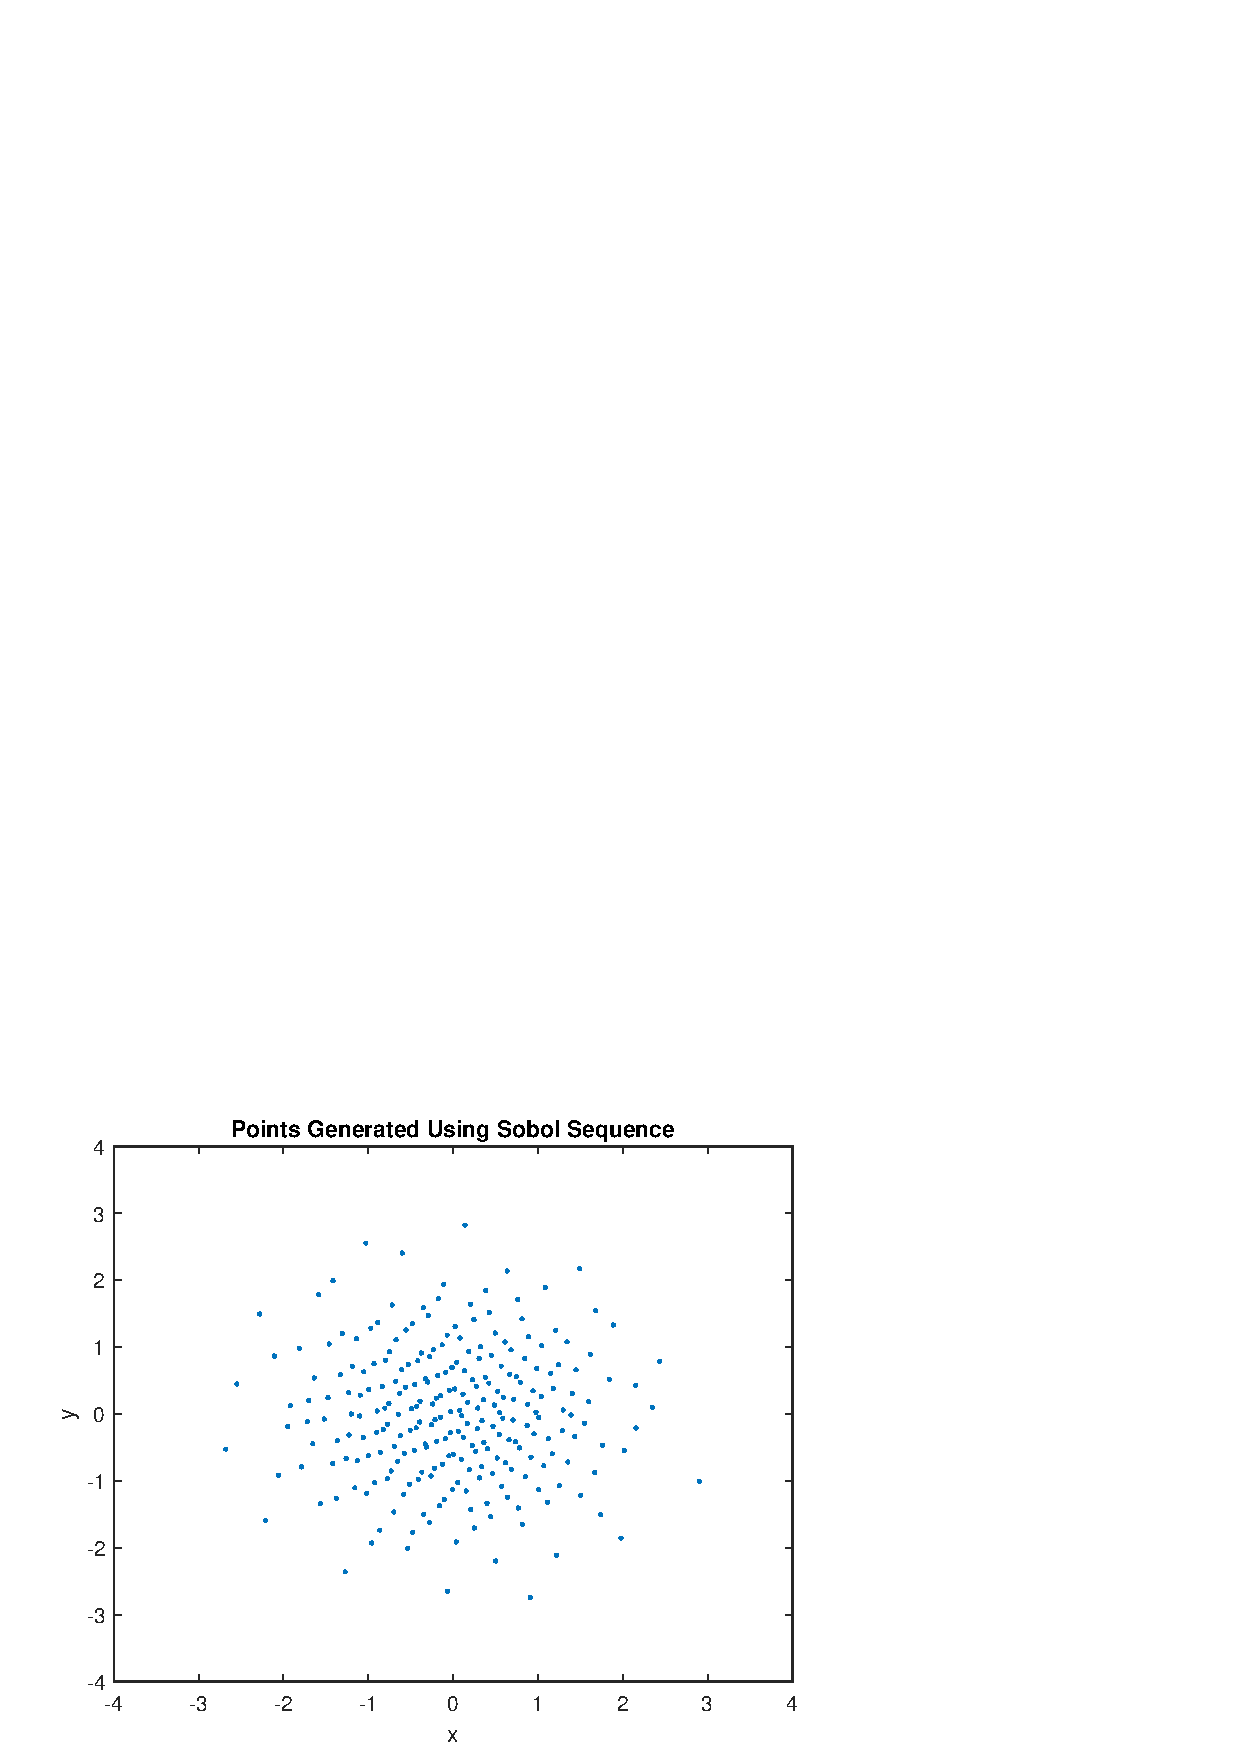
\includegraphics[width=0.7\textwidth]{SobolPoints}
\end{center}
\end{block}

\vspace{.1in}

\begin{block}{\Large \textbf{\blue {Model Problem}}}
\vspace{.1in}
\begin{itemize}
\item Bayesian inference is applied to logistic regression.

\vspace{.15in}

\item $t_i \sim \text{Ber} \left(\frac{\exp{\left(\beta_0+\sum_{j=1}^d\beta_j s_{ij}\right)}} {1+\exp \left({{\beta_0+\sum_{j=1}^d\beta_js_{ij}}}\right)}\right), \text{ for } i=1, 2, \dots , M$

\vspace{.15in}

\item Standard norm prior for $\boldsymbol{\beta}$

\vspace{.15in}

$\pi(\boldsymbol{b})=\frac{\exp{\left({-\frac{1}{2}\boldsymbol{b}^T\boldsymbol{b}}\right )}}{\sqrt{(2\pi)^{d+1}}}$

\vspace{.15in}

\item Posterior mean estimates of $\boldsymbol{\beta}$

\vspace{.15in}

 $\hat{\beta}_j=\frac{\int_{\mathbb{R}^{d+1}}b_jL(\boldsymbol{b})\pi(\boldsymbol{b})d\boldsymbol{b}}{\int_{\mathbb{R}^{d+1}}L(\boldsymbol{b})\pi(\boldsymbol{b})d\boldsymbol{b}} =: \frac{\mu_j}{\boldsymbol{\mu}}$, for $j=0, 1, 2,\ldots, d$

%\vspace{0.05in} 

%where $\hat{\beta}$ are the unknown parameters
\end{itemize}
\end{block}

\vspace{0.75in}

\begin{block}
{\small{\black{A special appreciation and thank you to the IIT College of Science for providing the funding behind this research project.}}}
\end{block}

\end{column}


\begin{column}{.015\linewidth} \end{column} %intercolumn space

\begin{column}{.31\linewidth}

\begin{block}{\Large \textbf{\blue {Choice of Density for Integration}}}
\vspace{.1in}
\begin{itemize}
\item $\mu_j/\boldsymbol{\mu}$ cannot be calculated analytically

\item Rewrite $\boldsymbol{\mu}$ as (similarly for $\mu_j$): 

\vspace{.15in}

$\boldsymbol{\mu}=\int_{\mathbb{R}^{d+1}}L(\boldsymbol{b})\pi(\boldsymbol{b})d\boldsymbol{b}=\int_{\mathbb{R}^{d+1}}\frac{L(\boldsymbol{b})\pi(\boldsymbol{b})}{\rho(\boldsymbol{b})}\rho(\boldsymbol{b})d\boldsymbol{b}=\int_{[0,1]^{d+1}}f(\boldsymbol{x})d\boldsymbol{x}$,

\vspace{.15in}

where $f(\boldsymbol{x})=f(\boldsymbol{R}(\boldsymbol{b}))=\frac{L(\boldsymbol{b})\pi(\boldsymbol{b})}{\rho(\boldsymbol{b})}$

\vspace{.15in}

and $\rho(\boldsymbol{b})=\left|d\boldsymbol{R}/d\boldsymbol{b}\right|$ for some suitable $\boldsymbol{R}:\mathbb{R}^{d+1}\rightarrow [0,1]^{d+1}$

\vspace{.1in}

\item Now, $\mu_j/\boldsymbol{\mu}$ can be approximated by sampling from $\rho(\boldsymbol{b})$ and applying quasi-Monte Carlo cubature

\item  We made the following choices for $\rho(\boldsymbol{b})$:
$\begin{array}{rrcl}
1) & \rho & = & \pi \\
2) & \rho & = & \rho_{\text{MLE}} = \text{Gaussian approximation to the}\\ 
&&&\hspace{4.5cm} \text{likelihood}\\
3) & \rho & \propto & \pi \cdot \rho_{\text{MLE}}
\end{array}$

\end{itemize}
\end{block}

\vspace{0.1in}

\begin{block}{\Large \textbf{\blue {New MATLAB Function}}}
\vspace{.1in}
\begin{itemize}

\item Developed  \alert{function} \mcode{BayesianInference} that \alert{automatically} estimates the unknown parameters $\hat{\boldsymbol{\beta}}$ using GAIL (Choi Et al, 2015)  

\item User inputs error tolerance, d, $\rho(\boldsymbol{b})$, and more

\end{itemize}
\end{block}

\vspace{0.1in}

\begin{block}{\Large \textbf{\blue {Uniform s-Data}}}    

\lstset{basicstyle=\small} 
\begin{lstlisting}  
M = 100; %number of s-Data values
s = (6+2)*rand(1,M)-2; % s-Data uniform in [-2,6]
dim=2; absTol=0.0005; n=5;
densityChoice = [true true true]; %Use all 3 densities
BayesianInference(M, s, dim, absTol, 
                 densityChoice,n)
\end{lstlisting}    

\vspace{.1in}

\begin{center}
\scalebox{0.7}{
\begin{tabular}{ |c|c|c| } 
 \hline
 Density & Runtime (seconds) & Samples Taken \\
 \hline 
 $\rho = \pi$ & 19.9122 & 655360\\
 $\rho = \rho_{\text{MLE}}$ & 0.91593 & 24576\\
 $\rho \propto \pi \cdot \rho_{\text{MLE}}$ & 0.99225 & 40960\\
 \hline
\end{tabular}
}
\end{center}

\vspace{.1in}

\begin{center}
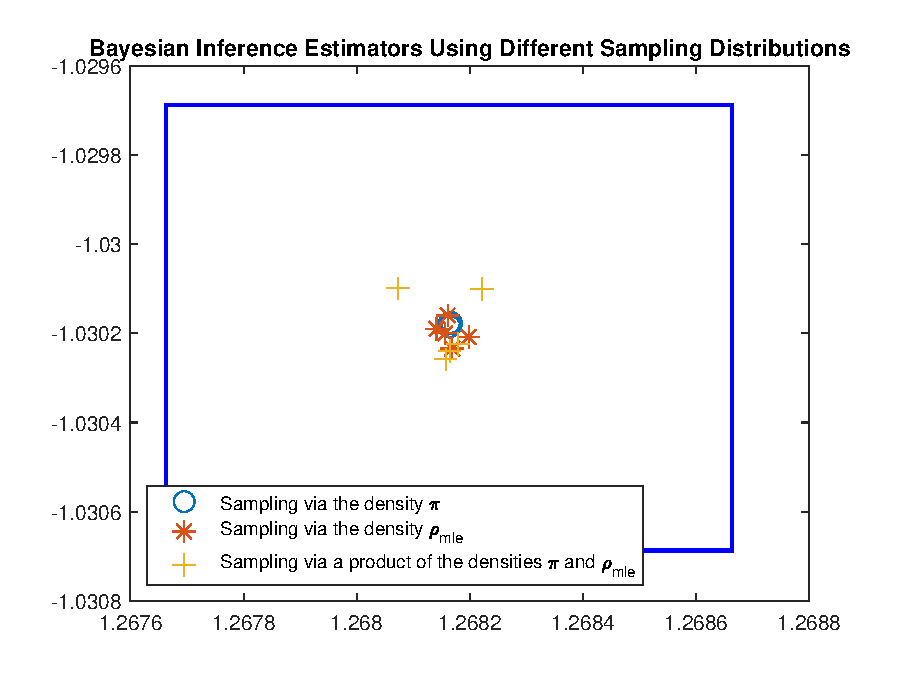
\includegraphics[width=0.7\textwidth]{UniformRandom}
\end{center} 
\end{block}
\end{column}

\begin{column}{.015\linewidth} \end{column} %intercolumn space

\begin{column}{.31\linewidth}
\begin{block}{\Large \textbf{\blue {Normal s-Data}}}    

\lstset{basicstyle=\small} 
\begin{lstlisting}      
M = 100; % number of s-Data values
s = 2.*randn(1,M)+2; % s-Data normal with mean and sd 2
dim=2; absTol=0.0005; n=5;
densityChoice = [true true true]; % Use all 3 densities
BayesianInference(M, s, dim, absTol, 
                 densityChoice,n)
\end{lstlisting}     

\vspace{.1in}

\begin{center}
\scalebox{0.7}{
\begin{tabular}{ |c|c|c| } 
 \hline
 Density & Runtime (seconds) & Samples Taken \\
 \hline 
 $\rho = \pi$ & 23.7317 & 589824\\
 $\rho = \rho_{\text{MLE}}$ & 0.78905 & 20480\\
 $\rho \propto \pi \cdot \rho_{\text{MLE}}$ & 1.0491 & 20480\\
 \hline
\end{tabular}
}
\end{center}

\vspace{.1in}

\begin{center}
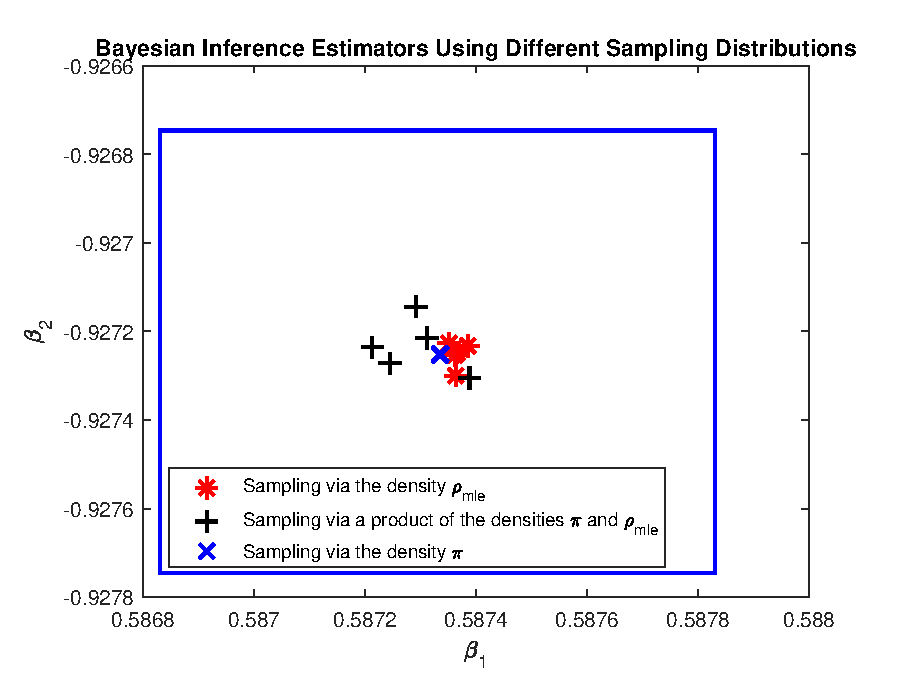
\includegraphics[width=0.7\textwidth]{NormalRandom}
\end{center} 

\end{block}

\bigskip

\begin{block}{\Large \textbf{\blue {Conclusions}}}

\vspace{.1in}

\begin{itemize}
\item Each density choice was successful in approximating posterior mean estimates within the desired tolerance level 

\item The choice of density directly affects the time taken 

\item Further work should be done to improve the run time of \mcode{BayesianInference} and generalize the function to solve a greater variety of problems

\item These results will be compared in detail to other methods used today, specifically Markov Chain Monte Carlo
\end{itemize}

\end{block}

\bigskip

\begin{block}{\Large \textbf{\blue {References}}}

\vspace{.1in}
\begin{itemize}
\item Choi, S.C.T., Ding, Y., Hickernell, F.J., Jiang, L., Jimenez Rugama,
Ll.A., Tong, X., Zhang,Y., Zhou, X. \emph{{GAIL}:
  {G}uaranteed {A}utomatic {I}ntegration {L}ibrary (version 2.1)}, MATLAB
  software, 2015.

\item Hickernell, F.J., Jimenez Rugama, Ll.A., Li, D. \textit{Contemporary Computational Mathematics --- A Celebration of the 80th Birthday of Ian Sloan.}  Adaptive Quasi-Monte Carlo Methods for Cubature. pages 597-619, Springer-Verlag, 2018.
\end{itemize}
\end{block}

\end{column}
\end{columns}

\end{frame}
\end{document}